\documentclass{article}\usepackage[]{graphicx}\usepackage[]{xcolor}
% maxwidth is the original width if it is less than linewidth
% otherwise use linewidth (to make sure the graphics do not exceed the margin)
\makeatletter
\def\maxwidth{ %
  \ifdim\Gin@nat@width>\linewidth
    \linewidth
  \else
    \Gin@nat@width
  \fi
}
\makeatother

\definecolor{fgcolor}{rgb}{0.345, 0.345, 0.345}
\newcommand{\hlnum}[1]{\textcolor[rgb]{0.686,0.059,0.569}{#1}}%
\newcommand{\hlsng}[1]{\textcolor[rgb]{0.192,0.494,0.8}{#1}}%
\newcommand{\hlcom}[1]{\textcolor[rgb]{0.678,0.584,0.686}{\textit{#1}}}%
\newcommand{\hlopt}[1]{\textcolor[rgb]{0,0,0}{#1}}%
\newcommand{\hldef}[1]{\textcolor[rgb]{0.345,0.345,0.345}{#1}}%
\newcommand{\hlkwa}[1]{\textcolor[rgb]{0.161,0.373,0.58}{\textbf{#1}}}%
\newcommand{\hlkwb}[1]{\textcolor[rgb]{0.69,0.353,0.396}{#1}}%
\newcommand{\hlkwc}[1]{\textcolor[rgb]{0.333,0.667,0.333}{#1}}%
\newcommand{\hlkwd}[1]{\textcolor[rgb]{0.737,0.353,0.396}{\textbf{#1}}}%
\let\hlipl\hlkwb

\usepackage{framed}
\makeatletter
\newenvironment{kframe}{%
 \def\at@end@of@kframe{}%
 \ifinner\ifhmode%
  \def\at@end@of@kframe{\end{minipage}}%
  \begin{minipage}{\columnwidth}%
 \fi\fi%
 \def\FrameCommand##1{\hskip\@totalleftmargin \hskip-\fboxsep
 \colorbox{shadecolor}{##1}\hskip-\fboxsep
     % There is no \\@totalrightmargin, so:
     \hskip-\linewidth \hskip-\@totalleftmargin \hskip\columnwidth}%
 \MakeFramed {\advance\hsize-\width
   \@totalleftmargin\z@ \linewidth\hsize
   \@setminipage}}%
 {\par\unskip\endMakeFramed%
 \at@end@of@kframe}
\makeatother

\definecolor{shadecolor}{rgb}{.97, .97, .97}
\definecolor{messagecolor}{rgb}{0, 0, 0}
\definecolor{warningcolor}{rgb}{1, 0, 1}
\definecolor{errorcolor}{rgb}{1, 0, 0}
\newenvironment{knitrout}{}{} % an empty environment to be redefined in TeX

\usepackage{alltt}
\usepackage[margin=1.0in]{geometry} % To set margins
\usepackage{amsmath}  % This allows me to use the align functionality.
                      % If you find yourself trying to replicate
                      % something you found online, ensure you're
                      % loading the necessary packages!
\usepackage{amsfonts} % Math font
\usepackage{fancyvrb}
\usepackage{hyperref} % For including hyperlinks
\usepackage[shortlabels]{enumitem}% For enumerated lists with labels specified
                    % We had to run tlmgr_install("enumitem") in R
\usepackage{float}    % For telling R where to put a table/figure
\usepackage{natbib}        %For the bibliography
\usepackage[skins,breakable]{tcolorbox}        %For the bibliography
\bibliographystyle{apalike}%For the bibliography
\IfFileExists{upquote.sty}{\usepackage{upquote}}{}
\begin{document}
\noindent\textbf{Homework 6: Regression}\\
\noindent\makebox[\linewidth]{\rule{\textwidth}{0.4pt}}
\noindent\underline{Submission Notes:} Please write your answers to each 
question under that question (not altogether at the end). It will be easier for 
me to give full credit if your answer is commented well, including comments 
about where you are completing each sub-part of the question. For an example,
see Homework 1.\\
\noindent\makebox[\linewidth]{\rule{\textwidth}{0.4pt}}


\begin{enumerate}
  %%%%%%%%%%%%%%%%%%%%%%%%%%%%%%%%%%%%%%%%%%%%%%%%%%%%%%%%%%%%%%%%%%%%%%%%%%%%%%
  %%%%%%%%%%%%%%%%%%%%%%%%%%%%%%%%%%%%%%%%%%%%%%%%%%%%%%%%%%%%%%%%%%%%%%%%%%%%%%
  % Question 1
  %%%%%%%%%%%%%%%%%%%%%%%%%%%%%%%%%%%%%%%%%%%%%%%%%%%%%%%%%%%%%%%%%%%%%%%%%%%%%%
  %%%%%%%%%%%%%%%%%%%%%%%%%%%%%%%%%%%%%%%%%%%%%%%%%%%%%%%%%%%%%%%%%%%%%%%%%%%%%%
  \item In Lecture 13, we discussed the linear algebra formulation of linear regression.
  For example, we can set up perfectly simulated regression data as follows:
\begin{knitrout}\scriptsize
\definecolor{shadecolor}{rgb}{0.969, 0.969, 0.969}\color{fgcolor}\begin{kframe}
\begin{alltt}
\hldef{simulate.reg} \hlkwb{<-} \hlkwa{function}\hldef{(}\hlkwc{n}\hldef{=}\hlnum{100}\hldef{,}
                         \hlkwc{betas}\hldef{=}\hlkwd{c}\hldef{(}\hlnum{4.35}\hldef{,} \hlnum{1.73}\hldef{,} \hlnum{0.02}\hldef{,} \hlnum{2.78}\hldef{),}
                         \hlkwc{sigma}\hldef{=}\hlnum{4.16}\hldef{,}
                         \hlkwc{set.seed}\hldef{=F)\{}
  \hlcom{# Specify Coefficients}
  \hldef{beta} \hlkwb{<-} \hlkwd{matrix}\hldef{(}\hlkwc{data} \hldef{= betas,} \hlkwc{nrow}\hldef{=}\hlnum{4}\hldef{)}
  \hlcom{# Specify Error Distribution}
  \hldef{mu.epsilon} \hlkwb{<-} \hlnum{0}
  \hldef{sigma.epsilon}\hlkwb{<-}\hlkwd{sqrt}\hldef{(sigma)}
  \hlcom{# Simulate Regression Data}
  \hlkwa{if}\hldef{(set.seed)\{}\hlkwd{set.seed}\hldef{(}\hlnum{7272}\hldef{)\}}
  \hldef{x1} \hlkwb{<-} \hlkwd{runif}\hldef{(}\hlkwc{n}\hldef{=n,} \hlkwc{min}\hldef{=}\hlopt{-}\hlnum{5}\hldef{,} \hlkwc{max}\hldef{=}\hlnum{5}\hldef{)}
  \hldef{x2} \hlkwb{<-} \hlkwd{runif}\hldef{(}\hlkwc{n}\hldef{=n,} \hlkwc{min}\hldef{=}\hlopt{-}\hlnum{5}\hldef{,} \hlkwc{max}\hldef{=}\hlnum{5}\hldef{)}
  \hldef{x} \hlkwb{<-} \hlkwd{cbind}\hldef{(}\hlnum{1}\hldef{, x1, x2, x1}\hlopt{*}\hldef{x2)}
  \hldef{epsilon} \hlkwb{<-} \hlkwd{rnorm}\hldef{(}\hlkwc{n}\hldef{=n,} \hlkwc{mean}\hldef{=}\hlnum{0}\hldef{,} \hlkwc{sd}\hldef{=sigma.epsilon)}
  \hldef{y} \hlkwb{<-} \hldef{x} \hlopt{%*%} \hldef{beta} \hlopt{+} \hldef{epsilon}
  \hlcom{# Return simulated data}
  \hldef{dat} \hlkwb{<-} \hlkwd{tibble}\hldef{(}\hlkwc{y}\hldef{=y,} \hlkwc{x1}\hldef{=x1,} \hlkwc{x2}\hldef{=x2)}
  \hlkwd{return}\hldef{(dat)}
\hldef{\}}
\end{alltt}
\end{kframe}
\end{knitrout}
  In Lecture 15, we discussed regression-based inference. During office hours, 
  I had some discussions about the mathematical statistics behind these results. 
  Although we don't do the real-analysis style derivations in this course that 
  we might in Mathematical Statistics, we have plenty of tools to investigate 
  these ideas numerically. Complete the parts below to conduct this exploration.
  \begin{enumerate}
    \item Use the \texttt{simulate.reg()} function to simulate regression data 
    using the default set of coefficients over a grid of $\sigma_\epsilon$ 
    values from $\sigma_\epsilon=0$ to $\sigma_\epsilon=5$. Compute the
    $SS_{res}$ and $SS_{reg}$ from the resulting regression model, and plot
    the points using color to denote the $\sigma_\epsilon$ value. Make sure you
    set \texttt{set.seed} to \texttt{T} so you can compare the output at
    fixed $\mathbf{x}$ and $\mathbf{Y}$. \textbf{Why do you see the pattern
    that emerges?}\\
    \textbf{Hint:} I found it was easier to manually compute $SS_{res}$ and
    $SS_{reg}$ than it was to extract them from the result of an \texttt{aov}
    call.
    
    \begin{figure}[H]
    \centering
    
\begin{knitrout}\scriptsize
\definecolor{shadecolor}{rgb}{0.969, 0.969, 0.969}\color{fgcolor}\begin{kframe}
\begin{alltt}
\hldef{asim} \hlkwb{<-} \hlkwd{tibble}\hldef{(}\hlkwc{sigma} \hldef{=} \hlkwd{rep}\hldef{(}\hlnum{NA}\hldef{,} \hlnum{1000}\hldef{),}
           \hlkwc{SSres} \hldef{=} \hlkwd{rep}\hldef{(}\hlnum{NA}\hldef{,} \hlnum{1000}\hldef{),}
           \hlkwc{SSreg} \hldef{=} \hlkwd{rep}\hldef{(}\hlnum{NA}\hldef{,} \hlnum{1000}\hldef{))}

\hldef{sigmas} \hlkwb{<-} \hlkwd{seq}\hldef{(}\hlkwc{from} \hldef{=} \hlnum{0}\hldef{,} \hlkwc{to} \hldef{=} \hlnum{5}\hldef{,} \hlkwc{length.out} \hldef{=} \hlnum{1000}\hldef{)}

\hlkwa{for}\hldef{(i} \hlkwa{in} \hlnum{1}\hlopt{:}\hlnum{1000}\hldef{)\{}

  \hldef{dat} \hlkwb{<-} \hlkwd{simulate.reg}\hldef{(}\hlkwc{sigma} \hldef{= sigmas[i],} \hlkwc{set.seed}\hldef{=T)}

  \hldef{asim}\hlopt{$}\hldef{sigma[i]} \hlkwb{<-} \hldef{sigmas[i]}

  \hldef{anova} \hlkwb{<-} \hlkwd{aov}\hldef{(y} \hlopt{~} \hldef{x1} \hlopt{+} \hldef{x2} \hlopt{+} \hldef{x1}\hlopt{*}\hldef{x2,} \hlkwc{data} \hldef{= dat)}

  \hldef{asim}\hlopt{$}\hldef{SSres[i]} \hlkwb{<-} \hlkwd{sum}\hldef{((anova}\hlopt{$}\hldef{residuals)}\hlopt{^}\hlnum{2}\hldef{)}

  \hldef{asim}\hlopt{$}\hldef{SSreg[i]} \hlkwb{<-} \hlkwd{sum}\hldef{((}\hlkwd{predict}\hldef{(anova)} \hlopt{-} \hlkwd{mean}\hldef{(dat}\hlopt{$}\hldef{y))}\hlopt{^}\hlnum{2}\hldef{)}

\hldef{\}}

\hlkwd{ggplot}\hldef{(}\hlkwc{data} \hldef{= asim,} \hlkwd{aes}\hldef{(}\hlkwc{x} \hldef{= SSres,} \hlkwc{y} \hldef{= SSreg,} \hlkwc{color} \hldef{= sigma))} \hlopt{+}
  \hlkwd{geom_point}\hldef{()} \hlopt{+}
  \hlkwd{xlab}\hldef{(}\hlkwd{bquote}\hldef{(SS[res]))} \hlopt{+}
  \hlkwd{ylab}\hldef{(}\hlkwd{bquote}\hldef{(SS[reg]))} \hlopt{+}
  \hlkwd{labs}\hldef{(}\hlkwc{color} \hldef{=} \hlkwd{bquote}\hldef{(sigma[epsilon]))} \hlopt{+}
  \hlkwd{theme_bw}\hldef{()}
\end{alltt}
\end{kframe}

\includegraphics[width=\maxwidth]{figure/unnamed-chunk-3-1} 
\end{knitrout}
    
    
    \label{sigma.fig}
    \caption{$\sigma$ across levels of $SS_{res}$ and $SS_{reg}$ (fixed $\mathbf{x}$ and $\mathbf{Y}$)}
    \end{figure}
    
    \textcolor{red}{We see that higher values of $SS_{res}$ and $SS_{reg}$ are associated with higher values of $\sigma_{\epsilon}$. This makes sense as $\sigma_{\epsilon}$ affects the variation around how the data fits the model, and higher variation in $\sigma_{\epsilon}$ will result in higher levels of variation in the regression residuals and against $\bar{Y}$.}
    
    \item Use the \texttt{simulate.reg()} function to simulate regression data 
    using the default set of coefficients. Create a plot that shows the 
    distribution of the $\beta$s. Make sure you set \texttt{set.seed} to 
    \texttt{F} so you can compare the output for differing samples of
    $\mathbf{x}$ and $\mathbf{Y}$. \textbf{What do you notice about their 
    distributions?}
    
    \begin{figure}[H]
    \centering
    
\begin{knitrout}\scriptsize
\definecolor{shadecolor}{rgb}{0.969, 0.969, 0.969}\color{fgcolor}\begin{kframe}
\begin{alltt}
\hldef{bsim} \hlkwb{<-} \hlkwd{tibble}\hldef{(}\hlkwc{Beta0} \hldef{=} \hlkwd{rep}\hldef{(}\hlnum{NA}\hldef{,} \hlnum{1000}\hldef{),}
           \hlkwc{Beta1} \hldef{=} \hlkwd{rep}\hldef{(}\hlnum{NA}\hldef{,} \hlnum{1000}\hldef{),}
           \hlkwc{Beta2} \hldef{=} \hlkwd{rep}\hldef{(}\hlnum{NA}\hldef{,} \hlnum{1000}\hldef{),}
           \hlkwc{Beta3} \hldef{=} \hlkwd{rep}\hldef{(}\hlnum{NA}\hldef{,} \hlnum{1000}\hldef{))}

\hlkwa{for} \hldef{(i} \hlkwa{in} \hlnum{1}\hlopt{:}\hlnum{1000}\hldef{)\{}

  \hldef{dat} \hlkwb{<-} \hlkwd{simulate.reg}\hldef{(}\hlkwc{set.seed}\hldef{=F)}

  \hldef{mod} \hlkwb{<-} \hlkwd{data.frame}\hldef{(}\hlkwd{summary}\hldef{(}\hlkwd{lm}\hldef{(y} \hlopt{~} \hldef{x1} \hlopt{+} \hldef{x2} \hlopt{+} \hldef{x1}\hlopt{*}\hldef{x2,} \hlkwc{data} \hldef{= dat))}\hlopt{$}\hldef{coefficients)}

  \hldef{bsim}\hlopt{$}\hldef{Beta0[i]} \hlkwb{<-} \hldef{mod}\hlopt{$}\hldef{Estimate[}\hlnum{1}\hldef{]}
  \hldef{bsim}\hlopt{$}\hldef{Beta1[i]} \hlkwb{<-} \hldef{mod}\hlopt{$}\hldef{Estimate[}\hlnum{2}\hldef{]}
  \hldef{bsim}\hlopt{$}\hldef{Beta2[i]} \hlkwb{<-} \hldef{mod}\hlopt{$}\hldef{Estimate[}\hlnum{3}\hldef{]}
  \hldef{bsim}\hlopt{$}\hldef{Beta3[i]} \hlkwb{<-} \hldef{mod}\hlopt{$}\hldef{Estimate[}\hlnum{4}\hldef{]}


\hldef{\}}

\hldef{bsim} \hlkwb{<-} \hldef{bsim |>}
  \hlkwd{pivot_longer}\hldef{(}\hlkwc{cols} \hldef{=} \hlkwd{colnames}\hldef{(bsim),}
           \hlkwc{names_to} \hldef{=} \hlsng{"Beta"}\hldef{,}
           \hlkwc{values_to} \hldef{=} \hlsng{"Value"}\hldef{)}


\hlkwd{library}\hldef{(ggridges)}
\hlkwd{ggplot}\hldef{(}\hlkwc{data} \hldef{= bsim,} \hlkwd{aes}\hldef{(}\hlkwc{x} \hldef{= Value,} \hlkwc{y} \hldef{=} \hlkwd{fct_rev}\hldef{(}\hlkwd{as.factor}\hldef{(Beta))))} \hlopt{+}
  \hlkwd{geom_density_ridges}\hldef{(}\hlkwc{alpha} \hldef{=} \hlnum{0.5}\hldef{)} \hlopt{+}
  \hlkwd{theme_bw}\hldef{()} \hlopt{+}
  \hlkwd{xlab}\hldef{(}\hlsng{"Estimate"}\hldef{)} \hlopt{+}
  \hlkwd{geom_hline}\hldef{(}\hlkwc{yintercept} \hldef{=} \hlnum{0}\hldef{)} \hlopt{+}
  \hlkwd{ylab}\hldef{(}\hlsng{''}\hldef{)} \hlopt{+}
  \hlkwd{scale_y_discrete}\hldef{(}
\hlkwc{labels} \hldef{=} \hlkwd{c}\hldef{(}
  \hlsng{"Beta0"} \hldef{=} \hlkwd{bquote}\hldef{(beta[}\hlnum{0}\hldef{]),}
  \hlsng{"Beta1"} \hldef{=} \hlkwd{bquote}\hldef{(beta[}\hlnum{1}\hldef{]),}
  \hlsng{"Beta2"} \hldef{=} \hlkwd{bquote}\hldef{(beta[}\hlnum{2}\hldef{]),}
  \hlsng{"Beta3"} \hldef{=} \hlkwd{bquote}\hldef{(beta[}\hlnum{3}\hldef{])}
\hldef{)}
  \hldef{)}
\end{alltt}
\end{kframe}

\includegraphics[width=\maxwidth]{figure/unnamed-chunk-4-1} 
\end{knitrout}
    
    \label{beta.dist}
    \caption{Distribution of the $\beta$ coefficients}
    
    \end{figure}
    
    \textcolor{red}{The spread of their distributions is very different. $\beta_{0}$ has the widest spread, followed by non-interaction terms $\beta_{1}$ and $\beta_{2}$. Then, the coefficient with the least spread is clearly the interaction term $\beta_{3}$}
    
    \item Use the \texttt{simulate.reg()} function to simulate regression data 
    using the default set of coefficients. Create a plot that shows the 
    distribution of the $\hat{y}$s at $x_1=3.6$ and $x_2=-1.9$. Make sure you 
    set \texttt{set.seed} to \texttt{F} so you can compare the output for 
    differing samples of $\mathbf{x}$ and $\mathbf{Y}$. \textbf{What do you 
    notice about the distribution?}
    
    \begin{figure}[H]
    \centering
    
\begin{knitrout}\scriptsize
\definecolor{shadecolor}{rgb}{0.969, 0.969, 0.969}\color{fgcolor}\begin{kframe}
\begin{alltt}
\hldef{csim} \hlkwb{<-} \hlkwd{tibble}\hldef{(}\hlkwc{yhat} \hldef{=} \hlkwd{rep}\hldef{(}\hlnum{NA}\hldef{,} \hlnum{1000}\hldef{))}

\hlkwa{for} \hldef{(i} \hlkwa{in} \hlnum{1}\hlopt{:}\hlnum{1000}\hldef{)\{}


  \hldef{dat} \hlkwb{<-} \hlkwd{simulate.reg}\hldef{(}\hlkwc{set.seed}\hldef{=F)}

  \hldef{mod} \hlkwb{<-} \hlkwd{data.frame}\hldef{(}\hlkwd{summary}\hldef{(}\hlkwd{lm}\hldef{(y} \hlopt{~} \hldef{x1} \hlopt{+} \hldef{x2} \hlopt{+} \hldef{x1}\hlopt{*}\hldef{x2,} \hlkwc{data} \hldef{= dat))}\hlopt{$}\hldef{coefficients)}

  \hldef{betas} \hlkwb{<-} \hldef{mod}\hlopt{$}\hldef{Estimate}

  \hldef{csim}\hlopt{$}\hldef{yhat[i]} \hlkwb{<-} \hldef{betas[}\hlnum{1}\hldef{]} \hlopt{+} \hlnum{3.6}\hlopt{*}\hldef{betas[}\hlnum{2}\hldef{]} \hlopt{-} \hlnum{1.9}\hlopt{*}\hldef{betas[}\hlnum{3}\hldef{]} \hlopt{-} \hlnum{3.6}\hlopt{*}\hlnum{1.9}\hlopt{*}\hldef{betas[}\hlnum{4}\hldef{]}

\hldef{\}}

\hldef{hist} \hlkwb{<-} \hlkwd{ggplot}\hldef{(}\hlkwc{data} \hldef{= csim,} \hlkwd{aes}\hldef{(}\hlkwc{x} \hldef{= yhat,} \hlkwc{y} \hldef{=} \hlkwd{after_stat}\hldef{(density)))} \hlopt{+}
  \hlkwd{geom_histogram}\hldef{(}\hlkwc{bins} \hldef{=} \hlnum{15}\hldef{,} \hlkwc{color} \hldef{=} \hlsng{"black"}\hldef{,} \hlkwc{fill} \hldef{=} \hlsng{"lightgrey"}\hldef{)} \hlopt{+}
  \hlkwd{theme_bw}\hldef{()} \hlopt{+}
  \hlkwd{geom_hline}\hldef{(}\hlkwc{yintercept} \hldef{=} \hlnum{0}\hldef{)} \hlopt{+}
  \hlkwd{xlab}\hldef{(}\hlkwd{bquote}\hldef{(}\hlkwd{hat}\hldef{(y)))} \hlopt{+}
  \hlkwd{ylab}\hldef{(}\hlsng{'Density'}\hldef{)}
  \hlkwd{scale_x_continuous}\hldef{(}\hlkwc{breaks} \hldef{=} \hlkwd{c}\hldef{(}\hlopt{-}\hlnum{10}\hldef{,} \hlopt{-}\hlnum{9}\hldef{,} \hlkwd{round}\hldef{(}\hlkwd{median}\hldef{(csim}\hlopt{$}\hldef{yhat),}\hlnum{2}\hldef{),} \hlopt{-}\hlnum{8}\hldef{,} \hlopt{-}\hlnum{7}\hldef{),} \hlkwc{limits} \hldef{=} \hlkwd{c}\hldef{(}\hlopt{-}\hlnum{10}\hldef{,}\hlopt{-}\hlnum{7}\hldef{))}
\end{alltt}
\begin{verbatim}
## <ScaleContinuousPosition>
##  Range:  
##  Limits:  -10 --   -7
\end{verbatim}
\begin{alltt}
\hldef{boxplot} \hlkwb{<-} \hlkwd{ggplot}\hldef{(}\hlkwc{data} \hldef{= csim,} \hlkwd{aes}\hldef{(}\hlkwc{x} \hldef{=} \hlsng{""}\hldef{,} \hlkwc{y} \hldef{= yhat))} \hlopt{+}
  \hlkwd{geom_boxplot}\hldef{()} \hlopt{+}
  \hlkwd{coord_flip}\hldef{()} \hlopt{+}
  \hlkwd{xlab}\hldef{(}\hlsng{''}\hldef{)} \hlopt{+}
  \hlkwd{ylab}\hldef{(}\hlkwd{bquote}\hldef{(}\hlkwd{hat}\hldef{(y)))} \hlopt{+}
  \hlkwd{theme_bw}\hldef{()} \hlopt{+}
  \hlkwd{scale_y_continuous}\hldef{(}\hlkwc{breaks} \hldef{=} \hlkwd{c}\hldef{(}\hlopt{-}\hlnum{10}\hldef{,} \hlopt{-}\hlnum{9}\hldef{,} \hlkwd{round}\hldef{(}\hlkwd{median}\hldef{(csim}\hlopt{$}\hldef{yhat),} \hlnum{2}\hldef{),} \hlopt{-}\hlnum{8}\hldef{,} \hlopt{-}\hlnum{7}\hldef{),} \hlkwc{limits} \hldef{=} \hlkwd{c}\hldef{(}\hlopt{-}\hlnum{10}\hldef{,}\hlopt{-}\hlnum{7}\hldef{))}

\hlkwd{library}\hldef{(patchwork)}
\hldef{hist} \hlopt{+} \hldef{boxplot} \hlopt{+}
  \hlkwd{plot_layout}\hldef{(}\hlkwc{nrow} \hldef{=} \hlnum{2}\hldef{,} \hlkwc{heights} \hldef{=} \hlkwd{c}\hldef{(}\hlnum{3}\hldef{,} \hlnum{1}\hldef{))}
\end{alltt}
\end{kframe}

\includegraphics[width=\maxwidth]{figure/unnamed-chunk-5-1} 
\end{knitrout}
    
    \label{predict.dist}
    \caption{Distribution of $\hat{y}$'s at $x_{1} = 3.6$ and $x_{2} = -1.9$}
    
    \end{figure}
    
    \textcolor{red}{The distribution of the $\hat{y}$ is Gaussian and centered at -8.5. The IQR is 0.53 [-8.74, -8.21] which is similar to the initial parameter $\sigma$.}
    
    \item Describe why using $t$-based inference makes sense when conducting 
    hypothesis tests or computing confidence intervals for a coefficient $\beta_j$, 
    and the conditional expectation or prediction of $Y$?
    
    \textcolor{red}{Based on the condition of linear regression that the residual $\epsilon$'s are normally distributed, the $\beta$'s are calculated off of fixed data and random gaussian $\epsilon$'s, so their distribution should be normal and therefore appropriate to $t$-test. Also based off of Figure: \ref{beta.dist}, we can see that each of the $\beta$'s are normally distributed in a simulated context. The same is true for for $\hat{y}$ in the way it's based off of fixed data and a normally distributed $\epsilon$, and is clearly normally distributed in Figure: \ref{predict.dist}.}
    
  \end{enumerate}
  %%%%%%%%%%%%%%%%%%%%%%%%%%%%%%%%%%%%%%%%%%%%%%%%%%%%%%%%%%%%%%%%%%%%%%%%%%%%%%
  %%%%%%%%%%%%%%%%%%%%%%%%%%%%%%%%%%%%%%%%%%%%%%%%%%%%%%%%%%%%%%%%%%%%%%%%%%%%%%
  % Question 2
  %%%%%%%%%%%%%%%%%%%%%%%%%%%%%%%%%%%%%%%%%%%%%%%%%%%%%%%%%%%%%%%%%%%%%%%%%%%%%%
  %%%%%%%%%%%%%%%%%%%%%%%%%%%%%%%%%%%%%%%%%%%%%%%%%%%%%%%%%%%%%%%%%%%%%%%%%%%%%%
  \item \cite{Su25} investigate how well-being of preschool teachers influences 
  the effort they put into managing their emotions at work (emotional labor).
  They found that how committed a teacher is to their career (career commitment)
  plays a key role in linking well-being to emotional labor, and this connection 
  gets stronger when they have more social support from colleagues or the community.\\

  As part of this work, they aimed to replicate findings that the level of social support moderates the impact of 
  preschool teachers' career commitment on emotional labor. Below, we will assess this piece to the puzzle.\\

  Fit a regression model predicting \texttt{Emotional Labor} using 
  \texttt{career commitment}, \texttt{social support}, and their interaction.
  Also include Gender, Age, and teaching experience.
  
\begin{knitrout}\scriptsize
\definecolor{shadecolor}{rgb}{0.969, 0.969, 0.969}\color{fgcolor}\begin{kframe}
\begin{alltt}
\hldef{dat} \hlkwb{<-} \hlkwd{read_csv}\hldef{(}\hlsng{'sudata-cleaned.csv'}\hldef{)}

\hldef{mod} \hlkwb{<-} \hlkwd{lm}\hldef{(EmotionalLabor} \hlopt{~} \hldef{CareerCommitment}\hlopt{*}\hldef{SocialSupport} \hlopt{+} \hldef{Gender} \hlopt{+} \hldef{Age} \hlopt{+} \hldef{TeachingExp,} \hlkwc{data} \hldef{= dat)}
\end{alltt}
\end{kframe}
\end{knitrout}
  
  \begin{enumerate}
    \item Perform a residual analysis. Do you have any concerns about the model
    fit?
    
    \begin{figure}[H]
    \centering

\begin{knitrout}\scriptsize
\definecolor{shadecolor}{rgb}{0.969, 0.969, 0.969}\color{fgcolor}\begin{kframe}
\begin{alltt}
\hlkwd{source}\hldef{(}\hlsng{'plotResiduals.R'}\hldef{)}
\hlkwd{source}\hldef{(}\hlsng{'plotInfluence.R'}\hldef{)}

\hlkwd{plotResiduals}\hldef{(mod)}
\end{alltt}
\end{kframe}

\includegraphics[width=\maxwidth]{figure/unnamed-chunk-7-1} 
\end{knitrout}
    
    \label{residual.plot}
    \caption{Residual Analysis of the Model}
    
    \end{figure}
    
    \textcolor{red}{The residuals fit a normal distribution well as indicated by the histogram and the qqplot. There are 3 residuals that are potentially unusually low, but otherwise the residuals are scattered irregularly as we'd hope. I'd say this is very typical for a regression model of this size.}
    
    \item Perform an analysis of leverage/influence. Do you have any concerns 
    about the model fit?
    
    \begin{figure}[H]
    \centering
    
\begin{knitrout}\scriptsize
\definecolor{shadecolor}{rgb}{0.969, 0.969, 0.969}\color{fgcolor}\begin{kframe}
\begin{alltt}
\hlkwd{plotInfluence}\hldef{(mod)}
\end{alltt}
\end{kframe}

\includegraphics[width=\maxwidth]{figure/unnamed-chunk-8-1} 
\end{knitrout}
    
    \label{influence.plot}
    \caption{Leverage/Influence analysis of the model}
    
    \end{figure}
    
    \textcolor{red}{There are several things to potentially be wary of here. There are 6-7 points with potentially high leverage, 4 points with large positive/negative DFFITs, and 3 points with large negative studentized residuals. For a positive, there are no points with large Cook's D. I'd maybe suggest testing a robust model to make sure these points don't heavily influence the model, but these results aren't super unusual for a model of this size.}
    
    \item Provide the results of the overall $F$ test. What does this tell you
    about the model you fit?
    
\begin{knitrout}\scriptsize
\definecolor{shadecolor}{rgb}{0.969, 0.969, 0.969}\color{fgcolor}\begin{kframe}
\begin{alltt}
\hlkwd{library}\hldef{(xtable)}
\hlkwd{library}\hldef{(effectsize)}

\hldef{ftest} \hlkwb{<-} \hlkwd{summary}\hldef{(}\hlkwd{aov}\hldef{(mod))[[}\hlnum{1}\hldef{]][}\hlopt{-}\hlnum{7}\hldef{,] |>}
  \hlkwd{mutate}\hldef{(}\hlkwc{significance} \hldef{=} \hlkwd{case_when}\hldef{(`Pr(>F)`} \hlopt{<} \hlnum{0.001} \hlopt{~} \hlsng{"***"}\hldef{,}
                              \hldef{`Pr(>F)`} \hlopt{>=} \hlnum{0.001} \hlopt{&} \hldef{`Pr(>F)`} \hlopt{<} \hlnum{0.01} \hlopt{~} \hlsng{"**"}\hldef{,}
                              \hldef{`Pr(>F)`} \hlopt{>=} \hlnum{0.01} \hlopt{&} \hldef{`Pr(>F)`} \hlopt{<} \hlnum{0.05} \hlopt{~} \hlsng{"*"}\hldef{,}
                              \hldef{`Pr(>F)`} \hlopt{>=} \hlnum{0.05} \hlopt{~} \hlsng{""}\hldef{),}
\hlkwc{omega2} \hldef{=} \hlkwd{omega_squared}\hldef{(mod)}\hlopt{$}\hldef{Omega2_partial,}
\hlkwc{interpretation} \hldef{=} \hlkwd{interpret_omega_squared}\hldef{(omega2,} \hlkwc{rules} \hldef{=} \hlsng{"cohen1992"}\hldef{))}

\hlkwd{colnames}\hldef{(ftest)} \hlkwb{<-} \hlkwd{c}\hldef{(}\hlsng{"df"}\hldef{,} \hlsng{"Sum Sq"}\hldef{,} \hlsng{"Mean Sq"}\hldef{,} \hlsng{"F"}\hldef{,} \hlsng{"p-value"}\hldef{,}
                 \hlsng{"Significance"}\hldef{,} \hlsng{"Effect Size"}\hldef{,} \hlsng{"Interpretation"}\hldef{)}
\hlkwd{rownames}\hldef{(ftest)} \hlkwb{<-} \hlkwd{c}\hldef{(}\hlsng{"Career Commitment"}\hldef{,} \hlsng{"Social Support"}\hldef{,} \hlsng{"Gender"}\hldef{,} \hlsng{"Age"}\hldef{,} \hlsng{"Teaching Experience"}\hldef{,}
                 \hlsng{"Career Commitment : Social Support"}\hldef{)}

\hldef{ftest}\hlopt{$}\hldef{`p-value`} \hlkwb{<-} \hlkwd{ifelse}\hldef{(ftest}\hlopt{$}\hldef{`p-value`} \hlopt{<} \hlnum{0.001}\hldef{,} \hlsng{'<0.001'}\hldef{,} \hlkwd{round}\hldef{(ftest}\hlopt{$}\hldef{`p-value`,} \hlnum{3}\hldef{))}

\hldef{ftest}\hlopt{$}\hldef{`Effect Size`} \hlkwb{<-} \hlkwd{ifelse}\hldef{(ftest}\hlopt{$}\hldef{`Effect Size`} \hlopt{==} \hlnum{0}\hldef{,} \hlsng{'<0.001'}\hldef{,} \hlkwd{round}\hldef{(ftest}\hlopt{$}\hldef{`Effect Size`,} \hlnum{3}\hldef{))}

\hldef{ftest} \hlkwb{<-} \hlkwd{xtable}\hldef{(ftest,}\hlkwc{label} \hldef{=} \hlsng{"model.f.tab"}\hldef{,} \hlkwc{caption} \hldef{=} \hlsng{"Model F-Test"}\hldef{,} \hlkwc{digits} \hldef{=} \hlnum{3}\hldef{)}
\end{alltt}
\end{kframe}
\end{knitrout}

% latex table generated in R 4.5.1 by xtable 1.8-4 package
% Sun Nov 16 22:33:05 2025
\begin{table}[H]
\centering
\begingroup\scriptsize
\begin{tabular}{lrrrrrrrr}
  \hline
 & df & Sum Sq & Mean Sq & F & p-value & Significance & Effect Size & Interpretation \\ 
  \hline
Career Commitment & 1.000 & 2657.030 & 2657.030 & 110.811 & $<$0.001 & *** & 0.235 & medium \\ 
  Social Support & 1.000 & 3.910 & 3.910 & 0.163 & 0.687 &  & $<$0.001 & very small \\ 
  Gender & 1.000 & 23.192 & 23.192 & 0.967 & 0.326 &  & $<$0.001 & very small \\ 
  Age & 1.000 & 1.290 & 1.290 & 0.054 & 0.817 &  & $<$0.001 & very small \\ 
  Teaching Experience & 1.000 & 91.652 & 91.652 & 3.822 & 0.051 &  & 0.008 & very small \\ 
  Career Commitment : Social Support & 1.000 & 186.770 & 186.770 & 7.789 & 0.006 & ** & 0.019 & very small \\ 
   \hline
\end{tabular}
\endgroup
\caption{Model F-Test} 
\label{model.f.tab}
\end{table}


\textcolor{red}{From the model fit, we see two terms that have a statistically discernible effect on Emotional Labor: Career Commitment ($F = 110.811$, $p < 0.001$, $\omega^2 = 0.235$) and the interaction between Career Commitment \& Social Support ($F = 7.789$, $p = 0.006$, $\omega^2 = 0.019$). We can clearly see that Career Commitment has a direct effect on Emotional Labor, but we'll need further probing to investigate what's going on with the interaction term.}

    
    \item Based on the model fit, does the amount of social support impact the 
    effect of career commitment on emotional labor?
    
\begin{knitrout}\scriptsize
\definecolor{shadecolor}{rgb}{0.969, 0.969, 0.969}\color{fgcolor}\begin{kframe}
\begin{alltt}
\hlcom{#Low Social Support}
\hldef{coef.low} \hlkwb{<-} \hlkwd{data.frame}\hldef{(}\hlkwd{t}\hldef{(}\hlkwd{coef}\hldef{(mod))) |>}   \hlcom{# A data frame of coefficients}
\hlkwd{mutate}\hldef{(}\hlkwc{X.Intercept.} \hldef{= X.Intercept.} \hlopt{+}
         \hldef{(}\hlkwd{mean}\hldef{(dat}\hlopt{$}\hldef{SocialSupport)}\hlopt{-}\hlkwd{sd}\hldef{(dat}\hlopt{$}\hldef{SocialSupport))} \hlopt{*} \hldef{SocialSupport,} \hlcom{# Adjust intercept and slope}
       \hlkwc{CareerCommitment} \hldef{= CareerCommitment} \hlopt{+}
         \hldef{(}\hlkwd{mean}\hldef{(dat}\hlopt{$}\hldef{SocialSupport)}\hlopt{-}\hlkwd{sd}\hldef{(dat}\hlopt{$}\hldef{SocialSupport))} \hlopt{*} \hldef{CareerCommitment.SocialSupport) |>}
\hldef{dplyr}\hlopt{::}\hlkwd{select}\hldef{(}\hlopt{-}\hlkwd{c}\hldef{(SocialSupport,CareerCommitment.SocialSupport))}

\hlcom{# When Social Support is average}
\hldef{coef.avg} \hlkwb{<-} \hlkwd{data.frame}\hldef{(}\hlkwd{t}\hldef{(}\hlkwd{coef}\hldef{(mod))) |>}  \hlcom{# A data frame of coefficients}
\hlkwd{mutate}\hldef{(}\hlkwc{X.Intercept.} \hldef{= X.Intercept.} \hlopt{+}
         \hldef{(}\hlkwd{mean}\hldef{(dat}\hlopt{$}\hldef{SocialSupport))} \hlopt{*} \hldef{SocialSupport,} \hlcom{# Adjust intercept and slope}
       \hlkwc{CareerCommitment} \hldef{= CareerCommitment}  \hlopt{+}
         \hldef{(}\hlkwd{mean}\hldef{(dat}\hlopt{$}\hldef{SocialSupport))} \hlopt{*} \hldef{CareerCommitment.SocialSupport)|>}
  \hldef{dplyr}\hlopt{::}\hlkwd{select}\hldef{(}\hlopt{-}\hlkwd{c}\hldef{(SocialSupport,CareerCommitment.SocialSupport))}

\hlcom{# High Social Support}
\hldef{coef.high} \hlkwb{<-} \hlkwd{data.frame}\hldef{(}\hlkwd{t}\hldef{(}\hlkwd{coef}\hldef{(mod))) |>} \hlcom{# A data frame of coefficients}
\hlkwd{mutate}\hldef{(}\hlkwc{X.Intercept.} \hldef{= X.Intercept.} \hlopt{+}
         \hldef{(}\hlkwd{mean}\hldef{(dat}\hlopt{$}\hldef{SocialSupport)}\hlopt{+}\hlkwd{sd}\hldef{(dat}\hlopt{$}\hldef{SocialSupport))} \hlopt{*} \hldef{SocialSupport,} \hlcom{# Adjust intercept and slope }
       \hlkwc{CareerCommitment} \hldef{= CareerCommitment} \hlopt{+}
         \hldef{(}\hlkwd{mean}\hldef{(dat}\hlopt{$}\hldef{SocialSupport)}\hlopt{+}\hlkwd{sd}\hldef{(dat}\hlopt{$}\hldef{SocialSupport))} \hlopt{*} \hldef{CareerCommitment.SocialSupport)|>}
  \hldef{dplyr}\hlopt{::}\hlkwd{select}\hldef{(}\hlopt{-}\hlkwd{c}\hldef{(SocialSupport,CareerCommitment.SocialSupport))}


\hldef{interaction_tab} \hlkwb{<-} \hlkwd{tibble}\hldef{(}\hlkwc{`Social Support Level`} \hldef{=} \hlkwd{c}\hldef{(}\hlsng{"low (-1 SD)"}\hldef{,} \hlsng{"average (mean)"}\hldef{,} \hlsng{"high (+1 SD)"}\hldef{),}
                      \hlkwc{`Career Commitment Slope  Estimate`} \hldef{=} \hlkwd{c}\hldef{(coef.low}\hlopt{$}\hldef{CareerCommitment,}
                                                       \hldef{coef.avg}\hlopt{$}\hldef{CareerCommitment,}
                                                       \hldef{coef.high}\hlopt{$}\hldef{CareerCommitment))}


\hldef{interaction_tab} \hlkwb{<-} \hlkwd{xtable}\hldef{(interaction_tab,}\hlkwc{label} \hldef{=} \hlsng{"interaction.tab"}\hldef{,} \hlkwc{caption} \hldef{=} \hlsng{"Career Commitment and Social Support Interaction Summary (Averaged Across Gender)"}\hldef{,} \hlkwc{digits} \hldef{=} \hlnum{3}\hldef{)}
\end{alltt}
\end{kframe}
\end{knitrout}
    
    
% latex table generated in R 4.5.1 by xtable 1.8-4 package
% Sun Nov 16 22:33:05 2025
\begin{table}[H]
\centering
\begingroup\normalsize
\begin{tabular}{lr}
  \hline
Social Support Level & Career Commitment Slope  Estimate \\ 
  \hline
low (-1 SD) & 0.284 \\ 
  average (mean) & 0.396 \\ 
  high (+1 SD) & 0.509 \\ 
   \hline
\end{tabular}
\endgroup
\caption{Career Commitment and Social Support Interaction Summary (Averaged Across Gender)} 
\label{interaction.tab}
\end{table}

    
    
    \textcolor{red}{We can see that the slope estimate of career commitment on emotional labor increases substantially as social support level increases.}
    
  \end{enumerate}
  %%%%%%%%%%%%%%%%%%%%%%%%%%%%%%%%%%%%%%%%%%%%%%%%%%%%%%%%%%%%%%%%%%%%%%%%%%%%%%
  %%%%%%%%%%%%%%%%%%%%%%%%%%%%%%%%%%%%%%%%%%%%%%%%%%%%%%%%%%%%%%%%%%%%%%%%%%%%%%
  % Question 3
  %%%%%%%%%%%%%%%%%%%%%%%%%%%%%%%%%%%%%%%%%%%%%%%%%%%%%%%%%%%%%%%%%%%%%%%%%%%%%%
  %%%%%%%%%%%%%%%%%%%%%%%%%%%%%%%%%%%%%%%%%%%%%%%%%%%%%%%%%%%%%%%%%%%%%%%%%%%%%%
  \item Continue with the regression from Question 2.
  \begin{enumerate}
    \item Use \texttt{emmeans()} from the \texttt{emmeans} package
    for \texttt{R} \citep{emmeans} to compute the estimated marginal means of
    \texttt{Emotional Labor} for low, average and high \texttt{career commitment}
    and \texttt{social support}. Report the results in a table and a figure.
    
    
\begin{knitrout}\scriptsize
\definecolor{shadecolor}{rgb}{0.969, 0.969, 0.969}\color{fgcolor}\begin{kframe}
\begin{alltt}
\hlkwd{library}\hldef{(emmeans)}

\hldef{emm} \hlkwb{<-} \hlkwd{data.frame}\hldef{(}\hlkwd{summary}\hldef{(}\hlkwd{emmeans}\hldef{(mod,} \hlopt{~} \hldef{CareerCommitment}\hlopt{*}\hldef{SocialSupport,}
           \hlkwc{at} \hldef{=} \hlkwd{list}\hldef{(}
             \hlkwc{CareerCommitment} \hldef{=} \hlkwd{c}\hldef{(}\hlkwd{mean}\hldef{(dat}\hlopt{$}\hldef{CareerCommitment)} \hlopt{-} \hlkwd{sd}\hldef{(dat}\hlopt{$}\hldef{CareerCommitment),}
                                  \hlkwd{mean}\hldef{(dat}\hlopt{$}\hldef{CareerCommitment),}
                                  \hlkwd{mean}\hldef{(dat}\hlopt{$}\hldef{CareerCommitment)} \hlopt{+} \hlkwd{sd}\hldef{(dat}\hlopt{$}\hldef{CareerCommitment)),}
             \hlkwc{SocialSupport} \hldef{=} \hlkwd{c}\hldef{(}\hlkwd{mean}\hldef{(dat}\hlopt{$}\hldef{SocialSupport)} \hlopt{-} \hlkwd{sd}\hldef{(dat}\hlopt{$}\hldef{SocialSupport),}
                               \hlkwd{mean}\hldef{(dat}\hlopt{$}\hldef{SocialSupport),}
                               \hlkwd{mean}\hldef{(dat}\hlopt{$}\hldef{SocialSupport)} \hlopt{+} \hlkwd{sd}\hldef{(dat}\hlopt{$}\hldef{SocialSupport))}
           \hldef{))))}


\hldef{emm_dat} \hlkwb{<-} \hlkwd{tibble}\hldef{(}\hlkwc{Career_Commitment} \hldef{=} \hlkwd{rep}\hldef{(}\hlkwd{c}\hldef{(}\hlsng{"Low"}\hldef{,} \hlsng{"Average"}\hldef{,} \hlsng{"High"}\hldef{),} \hlkwc{times} \hldef{=} \hlnum{3}\hldef{),}
              \hlkwc{Social_Support} \hldef{=} \hlkwd{rep}\hldef{(}\hlkwd{c}\hldef{(}\hlsng{"Low"}\hldef{,} \hlsng{"Average"}\hldef{,} \hlsng{"High"}\hldef{),} \hlkwc{each} \hldef{=} \hlnum{3}\hldef{),}
              \hlkwc{emmean} \hldef{= emm}\hlopt{$}\hldef{emmean,}
              \hlkwc{CI_low} \hldef{= emm}\hlopt{$}\hldef{lower.CL,}
              \hlkwc{CI_high} \hldef{= emm}\hlopt{$}\hldef{upper.CL) |>}
  \hlkwd{mutate}\hldef{(}\hlkwc{Career_Commitment} \hldef{=} \hlkwd{factor}\hldef{(Career_Commitment,} \hlkwc{levels} \hldef{=} \hlkwd{c}\hldef{(}\hlsng{"Low"}\hldef{,} \hlsng{"Average"}\hldef{,} \hlsng{"High"}\hldef{)),}
     \hlkwc{Social_Support} \hldef{=} \hlkwd{factor}\hldef{(Social_Support,} \hlkwc{levels} \hldef{=} \hlkwd{c}\hldef{(}\hlsng{"Low"}\hldef{,} \hlsng{"Average"}\hldef{,} \hlsng{"High"}\hldef{)))}


\hlkwd{colnames}\hldef{(emm)} \hlkwb{<-} \hlkwd{c}\hldef{(}\hlsng{"Career Commitment"}\hldef{,} \hlsng{"Social Support"}\hldef{,}
               \hlsng{"EMM of Emotional Labor"}\hldef{,} \hlsng{"SE"}\hldef{,}
               \hlsng{"df"}\hldef{,} \hlsng{"Lower CL"}\hldef{,} \hlsng{"Upper CL"}\hldef{)}


\hldef{emm} \hlkwb{<-} \hlkwd{xtable}\hldef{(emm,}\hlkwc{label} \hldef{=} \hlsng{"emm.tab"}\hldef{,} \hlkwc{caption} \hldef{=} \hlsng{"Estimated Marginal Means (Averaged Across Gender)"}\hldef{,} \hlkwc{digits} \hldef{=} \hlnum{3}\hldef{)}
\end{alltt}
\end{kframe}
\end{knitrout}
    
    
% latex table generated in R 4.5.1 by xtable 1.8-4 package
% Sun Nov 16 22:33:05 2025
\begin{table}[H]
\centering
\begingroup\normalsize
\begin{tabular}{rrrrrrr}
  \hline
Career Commitment & Social Support & EMM of Emotional Labor & SE & df & Lower CL & Upper CL \\ 
  \hline
17.445 & 31.429 & 35.565 & 0.585 & 350.000 & 34.414 & 36.716 \\ 
  24.036 & 31.429 & 37.434 & 0.549 & 350.000 & 36.355 & 38.514 \\ 
  30.626 & 31.429 & 39.304 & 0.767 & 350.000 & 37.796 & 40.812 \\ 
  17.445 & 38.934 & 34.955 & 0.566 & 350.000 & 33.842 & 36.068 \\ 
  24.036 & 38.934 & 37.566 & 0.501 & 350.000 & 36.580 & 38.552 \\ 
  30.626 & 38.934 & 40.177 & 0.583 & 350.000 & 39.029 & 41.324 \\ 
  17.445 & 46.438 & 34.345 & 0.766 & 350.000 & 32.838 & 35.852 \\ 
  24.036 & 46.438 & 37.697 & 0.613 & 350.000 & 36.492 & 38.902 \\ 
  30.626 & 46.438 & 41.049 & 0.659 & 350.000 & 39.753 & 42.345 \\ 
   \hline
\end{tabular}
\endgroup
\caption{Estimated Marginal Means (Averaged Across Gender)} 
\label{emm.tab}
\end{table}

 
 
 \begin{figure}[H]
 
 \centering
 
\begin{knitrout}\scriptsize
\definecolor{shadecolor}{rgb}{0.969, 0.969, 0.969}\color{fgcolor}\begin{kframe}
\begin{alltt}
\hlkwd{ggplot}\hldef{(}\hlkwc{data} \hldef{= emm_dat)} \hlopt{+}
  \hlkwd{geom_point}\hldef{(}\hlkwd{aes}\hldef{(}\hlkwc{x} \hldef{= Social_Support,}
                 \hlkwc{y} \hldef{= emmean,}
                 \hlkwc{color} \hldef{= Career_Commitment),}
             \hlkwc{position} \hldef{=} \hlkwd{position_dodge}\hldef{(}\hlkwc{width} \hldef{=} \hlnum{0.5}\hldef{))} \hlopt{+}
  \hlkwd{geom_errorbar}\hldef{(}\hlkwd{aes}\hldef{(}\hlkwc{x} \hldef{= Social_Support,}
                    \hlkwc{ymin}\hldef{=CI_low,}
                    \hlkwc{ymax} \hldef{= CI_high,}
                    \hlkwc{color} \hldef{= Career_Commitment),}
                \hlkwc{position} \hldef{=} \hlkwd{position_dodge}\hldef{(}\hlkwc{width} \hldef{=} \hlnum{0.5}\hldef{),}
                \hlkwc{width} \hldef{=} \hlnum{0.1}\hldef{)} \hlopt{+}
  \hlkwd{theme_bw}\hldef{()} \hlopt{+}
  \hlkwd{labs}\hldef{(}\hlkwc{x} \hldef{=} \hlsng{"Social Support"}\hldef{,}
       \hlkwc{y} \hldef{=} \hlsng{"Estimated Marginal Mean of Emotional Labor"}\hldef{,}
       \hlkwc{color} \hldef{=} \hlsng{"Career Commitment"}\hldef{)}
\end{alltt}
\end{kframe}
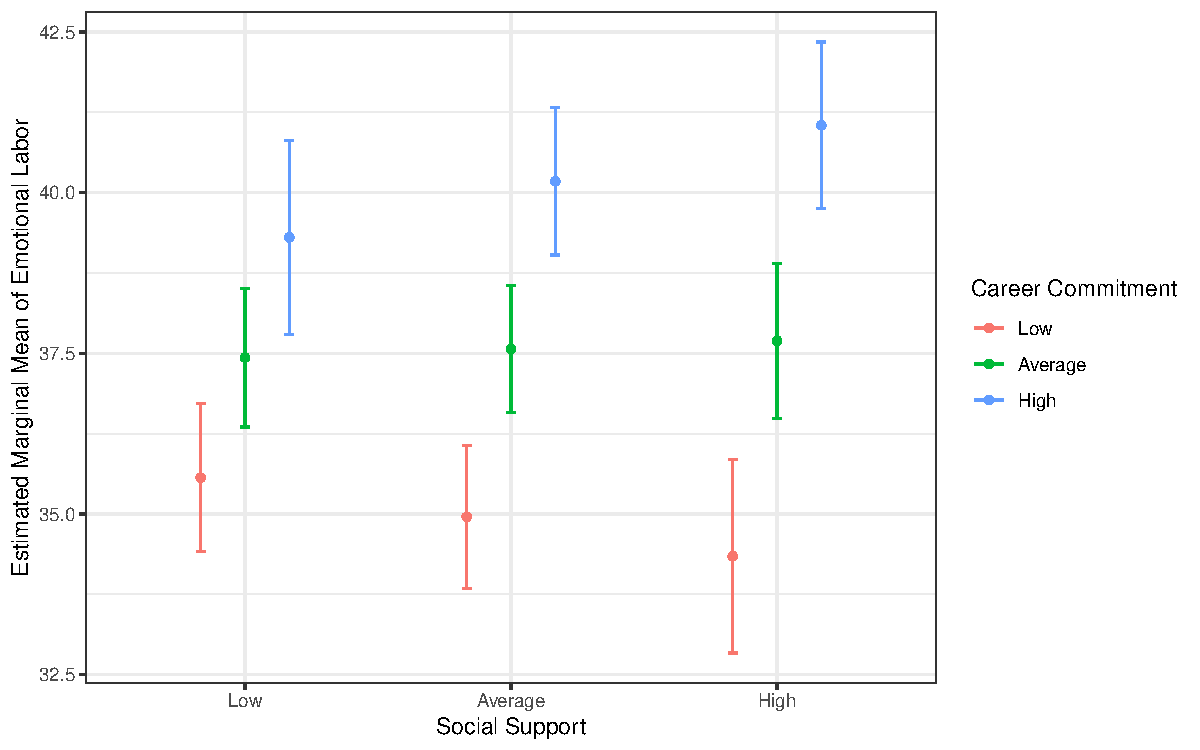
\includegraphics[width=\maxwidth]{figure/unnamed-chunk-15-1} 
\end{knitrout}
 
    \label{emm.plot}
    \caption{Estimated Marginal Means of Emotional Labor Across Low (Mean-SD), Average (Mean), and High (Mean+SD) Levels of Career Commitment and Social Support (Averaged Across Gender)}
    
    \end{figure}
    
    
    \item Use \texttt{emtrends()} from the \texttt{emmeans} package
    for \texttt{R} \citep{emmeans} to compute the slope for \texttt{career commitment}
    at low, average, and high \texttt{social support}. Report the results in a 
    table and use \texttt{ggeffect()} from the \texttt{ggeffects} package for
    \texttt{R} \citep{ggeffects} to create a plot. 
    
\begin{knitrout}\scriptsize
\definecolor{shadecolor}{rgb}{0.969, 0.969, 0.969}\color{fgcolor}\begin{kframe}
\begin{alltt}
\hldef{emt} \hlkwb{<-} \hlkwd{data.frame}\hldef{(}\hlkwd{test}\hldef{(}\hlkwd{emtrends}\hldef{(mod,} \hlopt{~} \hldef{CareerCommitment}\hlopt{*}\hldef{SocialSupport,} \hlkwc{var}\hldef{=}\hlsng{"CareerCommitment"}\hldef{,}
     \hlkwc{at} \hldef{=} \hlkwd{list}\hldef{(}\hlkwc{SocialSupport} \hldef{=} \hlkwd{c}\hldef{(}\hlkwd{mean}\hldef{(dat}\hlopt{$}\hldef{SocialSupport)} \hlopt{-} \hlkwd{sd}\hldef{(dat}\hlopt{$}\hldef{SocialSupport),}
                                 \hlkwd{mean}\hldef{(dat}\hlopt{$}\hldef{SocialSupport),}
                                 \hlkwd{mean}\hldef{(dat}\hlopt{$}\hldef{SocialSupport)} \hlopt{+} \hlkwd{sd}\hldef{(dat}\hlopt{$}\hldef{SocialSupport))))))}


\hlkwd{colnames}\hldef{(emt)} \hlkwb{<-} \hlkwd{c}\hldef{(}\hlsng{"Career Commitment"}\hldef{,} \hlsng{"Social Support"}\hldef{,}
               \hlsng{"Career Commitment Slope"}\hldef{,} \hlsng{"SE"}\hldef{,}
               \hlsng{"df"}\hldef{,} \hlsng{"t"}\hldef{,} \hlsng{"p-value"}\hldef{)}

\hldef{emt}\hlopt{$}\hldef{`p-value`} \hlkwb{<-} \hlkwd{ifelse}\hldef{(emt}\hlopt{$}\hldef{`p-value`} \hlopt{<} \hlnum{0.001}\hldef{,} \hlsng{"< 0.001"}\hldef{, emt}\hlopt{$}\hldef{`p-value`)}

\hldef{emt} \hlkwb{<-} \hlkwd{xtable}\hldef{(emt,}\hlkwc{label} \hldef{=} \hlsng{"emt.tab"}\hldef{,} \hlkwc{caption} \hldef{=} \hlsng{"Estimated Marginal Slope of Career Commitment 
Across Low (Mean-SD), Average (Mean), and High (Mean+SD)
          Levels of Social Support (Averaged
          Across Gender)"}\hldef{,} \hlkwc{digits} \hldef{=} \hlnum{3}\hldef{)}
\end{alltt}
\end{kframe}
\end{knitrout}
    
    
% latex table generated in R 4.5.1 by xtable 1.8-4 package
% Sun Nov 16 22:33:05 2025
\begin{table}[H]
\centering
\begingroup\normalsize
\begin{tabular}{rrrrrrl}
  \hline
Career Commitment & Social Support & Career Commitment Slope & SE & df & t & p-value \\ 
  \hline
23.994 & 31.429 & 0.284 & 0.061 & 350.000 & 4.614 & $<$ 0.001 \\ 
  23.994 & 38.934 & 0.396 & 0.043 & 350.000 & 9.278 & $<$ 0.001 \\ 
  23.994 & 46.438 & 0.509 & 0.056 & 350.000 & 9.114 & $<$ 0.001 \\ 
   \hline
\end{tabular}
\endgroup
\caption{Estimated Marginal Slope of Career Commitment 
Across Low (Mean-SD), Average (Mean), and High (Mean+SD)
          Levels of Social Support (Averaged
          Across Gender)} 
\label{emt.tab}
\end{table}


\begin{figure}[H]
\centering

\begin{knitrout}\scriptsize
\definecolor{shadecolor}{rgb}{0.969, 0.969, 0.969}\color{fgcolor}\begin{kframe}
\begin{alltt}
\hlkwd{library}\hldef{(ggeffects)}

\hldef{ggeff} \hlkwb{<-} \hlkwd{ggeffect}\hldef{(mod,} \hlopt{~} \hldef{CareerCommitment}\hlopt{*}\hldef{SocialSupport,}
                        \hlkwc{at} \hldef{=} \hlkwd{list}\hldef{(}\hlkwc{SocialSupport} \hldef{=} \hlkwd{c}\hldef{(}\hlkwd{mean}\hldef{(dat}\hlopt{$}\hldef{SocialSupport)} \hlopt{-} \hlkwd{sd}\hldef{(dat}\hlopt{$}\hldef{SocialSupport),}
                                     \hlkwd{mean}\hldef{(dat}\hlopt{$}\hldef{SocialSupport),}
                                     \hlkwd{mean}\hldef{(dat}\hlopt{$}\hldef{SocialSupport)} \hlopt{+} \hlkwd{sd}\hldef{(dat}\hlopt{$}\hldef{SocialSupport)))) |>}
  \hlkwd{tibble}\hldef{()}

\hlkwd{ggplot}\hldef{(}\hlkwc{data}\hldef{=ggeff)}\hlopt{+}
  \hlkwd{geom_line}\hldef{(}\hlkwd{aes}\hldef{(}\hlkwc{x}\hldef{=x,} \hlkwc{y}\hldef{=predicted,} \hlkwc{color}\hldef{=group))}\hlopt{+}
  \hlkwd{geom_ribbon}\hldef{(}\hlkwd{aes}\hldef{(}\hlkwc{x}\hldef{=x,} \hlkwc{ymin}\hldef{=conf.low,} \hlkwc{ymax}\hldef{=conf.high,} \hlkwc{fill}\hldef{=group),}
              \hlkwc{alpha}\hldef{=}\hlnum{0.1}\hldef{)}\hlopt{+}
  \hlkwd{theme_bw}\hldef{()}\hlopt{+}
  \hlkwd{ylab}\hldef{(}\hlsng{"Predicted Emotional Labor"}\hldef{)} \hlopt{+}
  \hlkwd{xlab}\hldef{(}\hlsng{"Career Commitment"}\hldef{)} \hlopt{+}
  \hlkwd{scale_color_discrete}\hldef{(}\hlsng{"Social Support"}\hldef{,} \hlkwc{labels} \hldef{=} \hlkwd{c}\hldef{(}\hlsng{"Low"}\hldef{,} \hlsng{"Average"}\hldef{,} \hlsng{"High"}\hldef{))} \hlopt{+}
  \hlkwd{guides}\hldef{(}\hlkwc{fill} \hldef{=} \hlsng{"none"}\hldef{)} \hlopt{+}
  \hlkwd{labs}\hldef{(}\hlkwc{color} \hldef{=} \hlsng{"Social Support"}\hldef{)}
\end{alltt}
\end{kframe}

\includegraphics[width=\maxwidth]{figure/unnamed-chunk-18-1} 
\end{knitrout}

\label{emt.plot}
\caption{Marginal Trend of Career Commitment across Low(Mean-SD), Average(Mean), and High(Mean+SD) Levels of Social Support (Averaged Across Gender)}

\end{figure}
    
    
    \item Use \texttt{pairs()} to compare the slopes for \texttt{career commitment}
    at low, average, and high \texttt{social support}. What does this tell us?
    
    
\begin{knitrout}\scriptsize
\definecolor{shadecolor}{rgb}{0.969, 0.969, 0.969}\color{fgcolor}\begin{kframe}
\begin{alltt}
\hldef{pairs} \hlkwb{<-} \hlkwd{data.frame}\hldef{(}\hlkwd{summary}\hldef{(}\hlkwd{pairs}\hldef{(}\hlkwd{emtrends}\hldef{(mod,} \hlopt{~} \hldef{CareerCommitment}\hlopt{*}\hldef{SocialSupport,} \hlkwc{var}\hldef{=}\hlsng{"CareerCommitment"}\hldef{,}
           \hlkwc{at} \hldef{=} \hlkwd{list}\hldef{(}\hlkwc{SocialSupport} \hldef{=} \hlkwd{c}\hldef{(}\hlkwd{mean}\hldef{(dat}\hlopt{$}\hldef{SocialSupport)}\hlopt{-}\hlkwd{sd}\hldef{(dat}\hlopt{$}\hldef{SocialSupport),}
                                       \hlkwd{mean}\hldef{(dat}\hlopt{$}\hldef{SocialSupport),}
                                       \hlkwd{mean}\hldef{(dat}\hlopt{$}\hldef{SocialSupport)} \hlopt{+} \hlkwd{sd}\hldef{(dat}\hlopt{$}\hldef{SocialSupport)))))))}

\hldef{pairs}\hlopt{$}\hldef{contrast} \hlkwb{<-} \hlkwd{c}\hldef{(}\hlsng{"Low - Average"}\hldef{,} \hlsng{"Low - High"}\hldef{,} \hlsng{"Average - High"}\hldef{)}

\hlkwd{colnames}\hldef{(pairs)} \hlkwb{<-} \hlkwd{c}\hldef{(}\hlsng{"Contrast (Social Support)"}\hldef{,} \hlsng{"Slope Difference"}\hldef{,}
                 \hlsng{"SE"}\hldef{,} \hlsng{"df"}\hldef{,}
                 \hlsng{"t"}\hldef{,} \hlsng{"p-value"}\hldef{)}


\hldef{pairs} \hlkwb{<-} \hlkwd{xtable}\hldef{(pairs,}\hlkwc{label} \hldef{=} \hlsng{"pairs.tab"}\hldef{,} \hlkwc{caption} \hldef{=} \hlsng{"Contrasts of Career Commitment Slopes at 
            Low(Mean-SD), Average(Mean), 
            and High(Mean+SD) Levels of Social Support (Averaged Across Gender)"}\hldef{,} \hlkwc{digits} \hldef{=} \hlnum{3}\hldef{)}
\end{alltt}
\end{kframe}
\end{knitrout}


% latex table generated in R 4.5.1 by xtable 1.8-4 package
% Sun Nov 16 22:33:06 2025
\begin{table}[H]
\centering
\begingroup\normalsize
\begin{tabular}{lrrrrr}
  \hline
Contrast (Social Support) & Slope Difference & SE & df & t & p-value \\ 
  \hline
Low - Average & -0.112 & 0.040 & 350.000 & -2.791 & 0.015 \\ 
  Low - High & -0.225 & 0.081 & 350.000 & -2.791 & 0.015 \\ 
  Average - High & -0.112 & 0.040 & 350.000 & -2.791 & 0.015 \\ 
   \hline
\end{tabular}
\endgroup
\caption{Contrasts of Career Commitment Slopes at 
            Low(Mean-SD), Average(Mean), 
            and High(Mean+SD) Levels of Social Support (Averaged Across Gender)} 
\label{pairs.tab}
\end{table}

    
    
    \textcolor{red}{Each of the pairwise comparisons of Career Commitment slopes is discernibly different, indicating that the effect of Social Support on Career Commitment generally extends far across every of Social Support. There isn't, for example, a point where the effect of Social Support on Career Commitment doesn't seem to make much of a difference anymore, the effect is pretty linear across the whole model.}
    
    \item Use \texttt{johnson\_neyman()} from the \texttt{interactions} package
    for \texttt{R} \citep{interactions} to evaluate which values of 
    \text{social suppport} yield slopes for  \texttt{career commitment} that
    are statistically discernible from zero. What does this tell us?
    
    \begin{figure}[H]
    \centering
    
\begin{knitrout}\scriptsize
\definecolor{shadecolor}{rgb}{0.969, 0.969, 0.969}\color{fgcolor}\begin{kframe}
\begin{alltt}
\hlkwd{library}\hldef{(interactions)}
\hlkwd{johnson_neyman}\hldef{(mod,}
                         \hlkwc{pred}\hldef{=}\hlsng{"CareerCommitment"}\hldef{,} \hlkwc{modx}\hldef{=}\hlsng{"SocialSupport"}\hldef{,}
                         \hlkwc{control.fdr} \hldef{= T,}
   \hlkwc{modx.label} \hldef{=} \hlsng{"Social Support"}\hldef{,}
   \hlkwc{y.label} \hldef{=} \hlsng{"Slope of Career Commitment"}\hldef{)}
\end{alltt}
\begin{verbatim}
## JOHNSON-NEYMAN INTERVAL
## 
## When SocialSupport is OUTSIDE the interval [-63.81, 24.86], the slope of
## CareerCommitment is p < .05.
## 
## Note: The range of observed values of SocialSupport is [18.00, 56.00]
## 
## Interval calculated using false discovery rate adjusted t = 2.05
\end{verbatim}
\end{kframe}
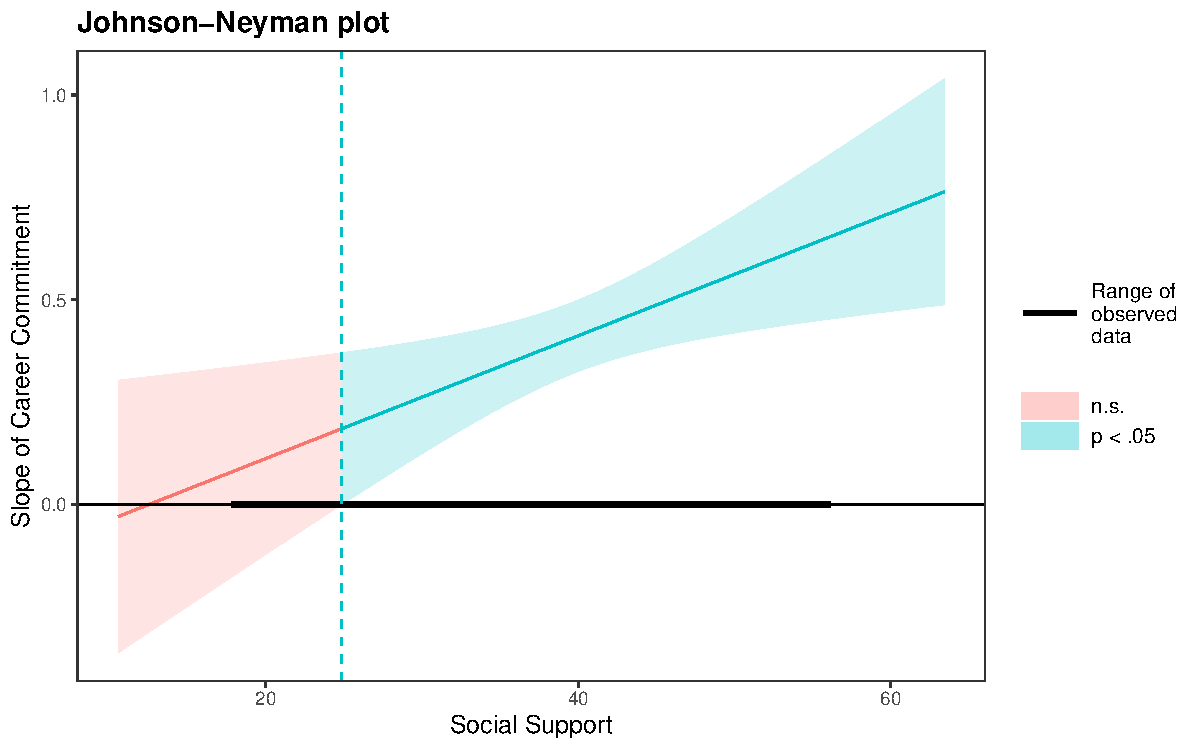
\includegraphics[width=\maxwidth]{figure/unnamed-chunk-21-1} 
\end{knitrout}
    
    \label{jn.plot}
    \caption{Johnson-Neyman Plot of Statistical Discernibility of the Slope of Career Commitment Across Values of Social Support (Averaged Across Gender)}
    
    \end{figure}
    
    \textcolor{red}{From the Johnson-Neyman plot, we can see that in the range of our observed data, the effect of Career Commitment on Emotional Labor is significant for levels of Social Support $> 24.86$. The slope of Career Commitment is linearly monotone increasing as well, which suggests that the effect of Career Commitment on Emotional Labor is heavily impacted by having a high level of Social Support and for people in the sample with low levels of Social Support, their Career Commitment doesn't discernibly affect their Emotional Labor.}
    
  \end{enumerate}
\end{enumerate}
\bibliography{bib}
\end{document}
